\chapter{Results}
\label{chap:results}

The learning from basic CNN model at the end of second stage are shown in Fig~\ref{fig:trainCNN} and \ref{fig:trainValCNN}. To improve on this basic CNN model, 81 variants have been tried on less number of iterations (epochs) being under resource constraints \ref{fig:gridSearchCNN10epoch}. As examples in Fig~\ref{fig:example6TP5FN} and \ref{fig:example1FP}, the results from detection stage that classify an object as a car are shown as orange line bounding boxes whereas red dot reveals the ground truth. For reference, A red dot inside bounding box means TP (True Positive), red dot without bounding box means FN (False Negative) and bounding box without any red dot inside means FP (False Positive). There are few cars that have been marked white, these are the masks that were applied to ignore objects that are irrelevant to the problem because of much distance and obstructions in view. CSI Analysis is shown in Figure~\ref{fig:100rowCSI} for the detection stage for YOLO and ResNet (RetinaNet) with different DPT over 100 randomly sampled rows from database.


\begin{figure}
\centering
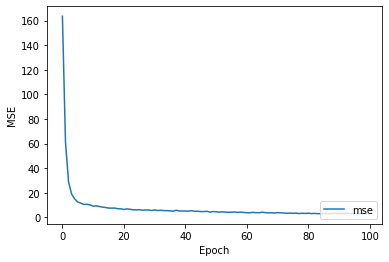
\includegraphics{images/train-1M-data-1000-epoch.png}
\caption{Training learning curve with mean squared error over 1000 epochs}
\label{fig:trainCNN}
\end{figure} 

\begin{figure}
\centering
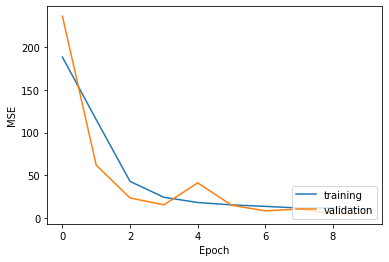
\includegraphics{images/train-val-1M-data-10-epoch.png}
\caption{Training with validation, mean square error over 10 epochs}
\label{fig:trainValCNN}
\end{figure} 

\begin{figure}
\centering
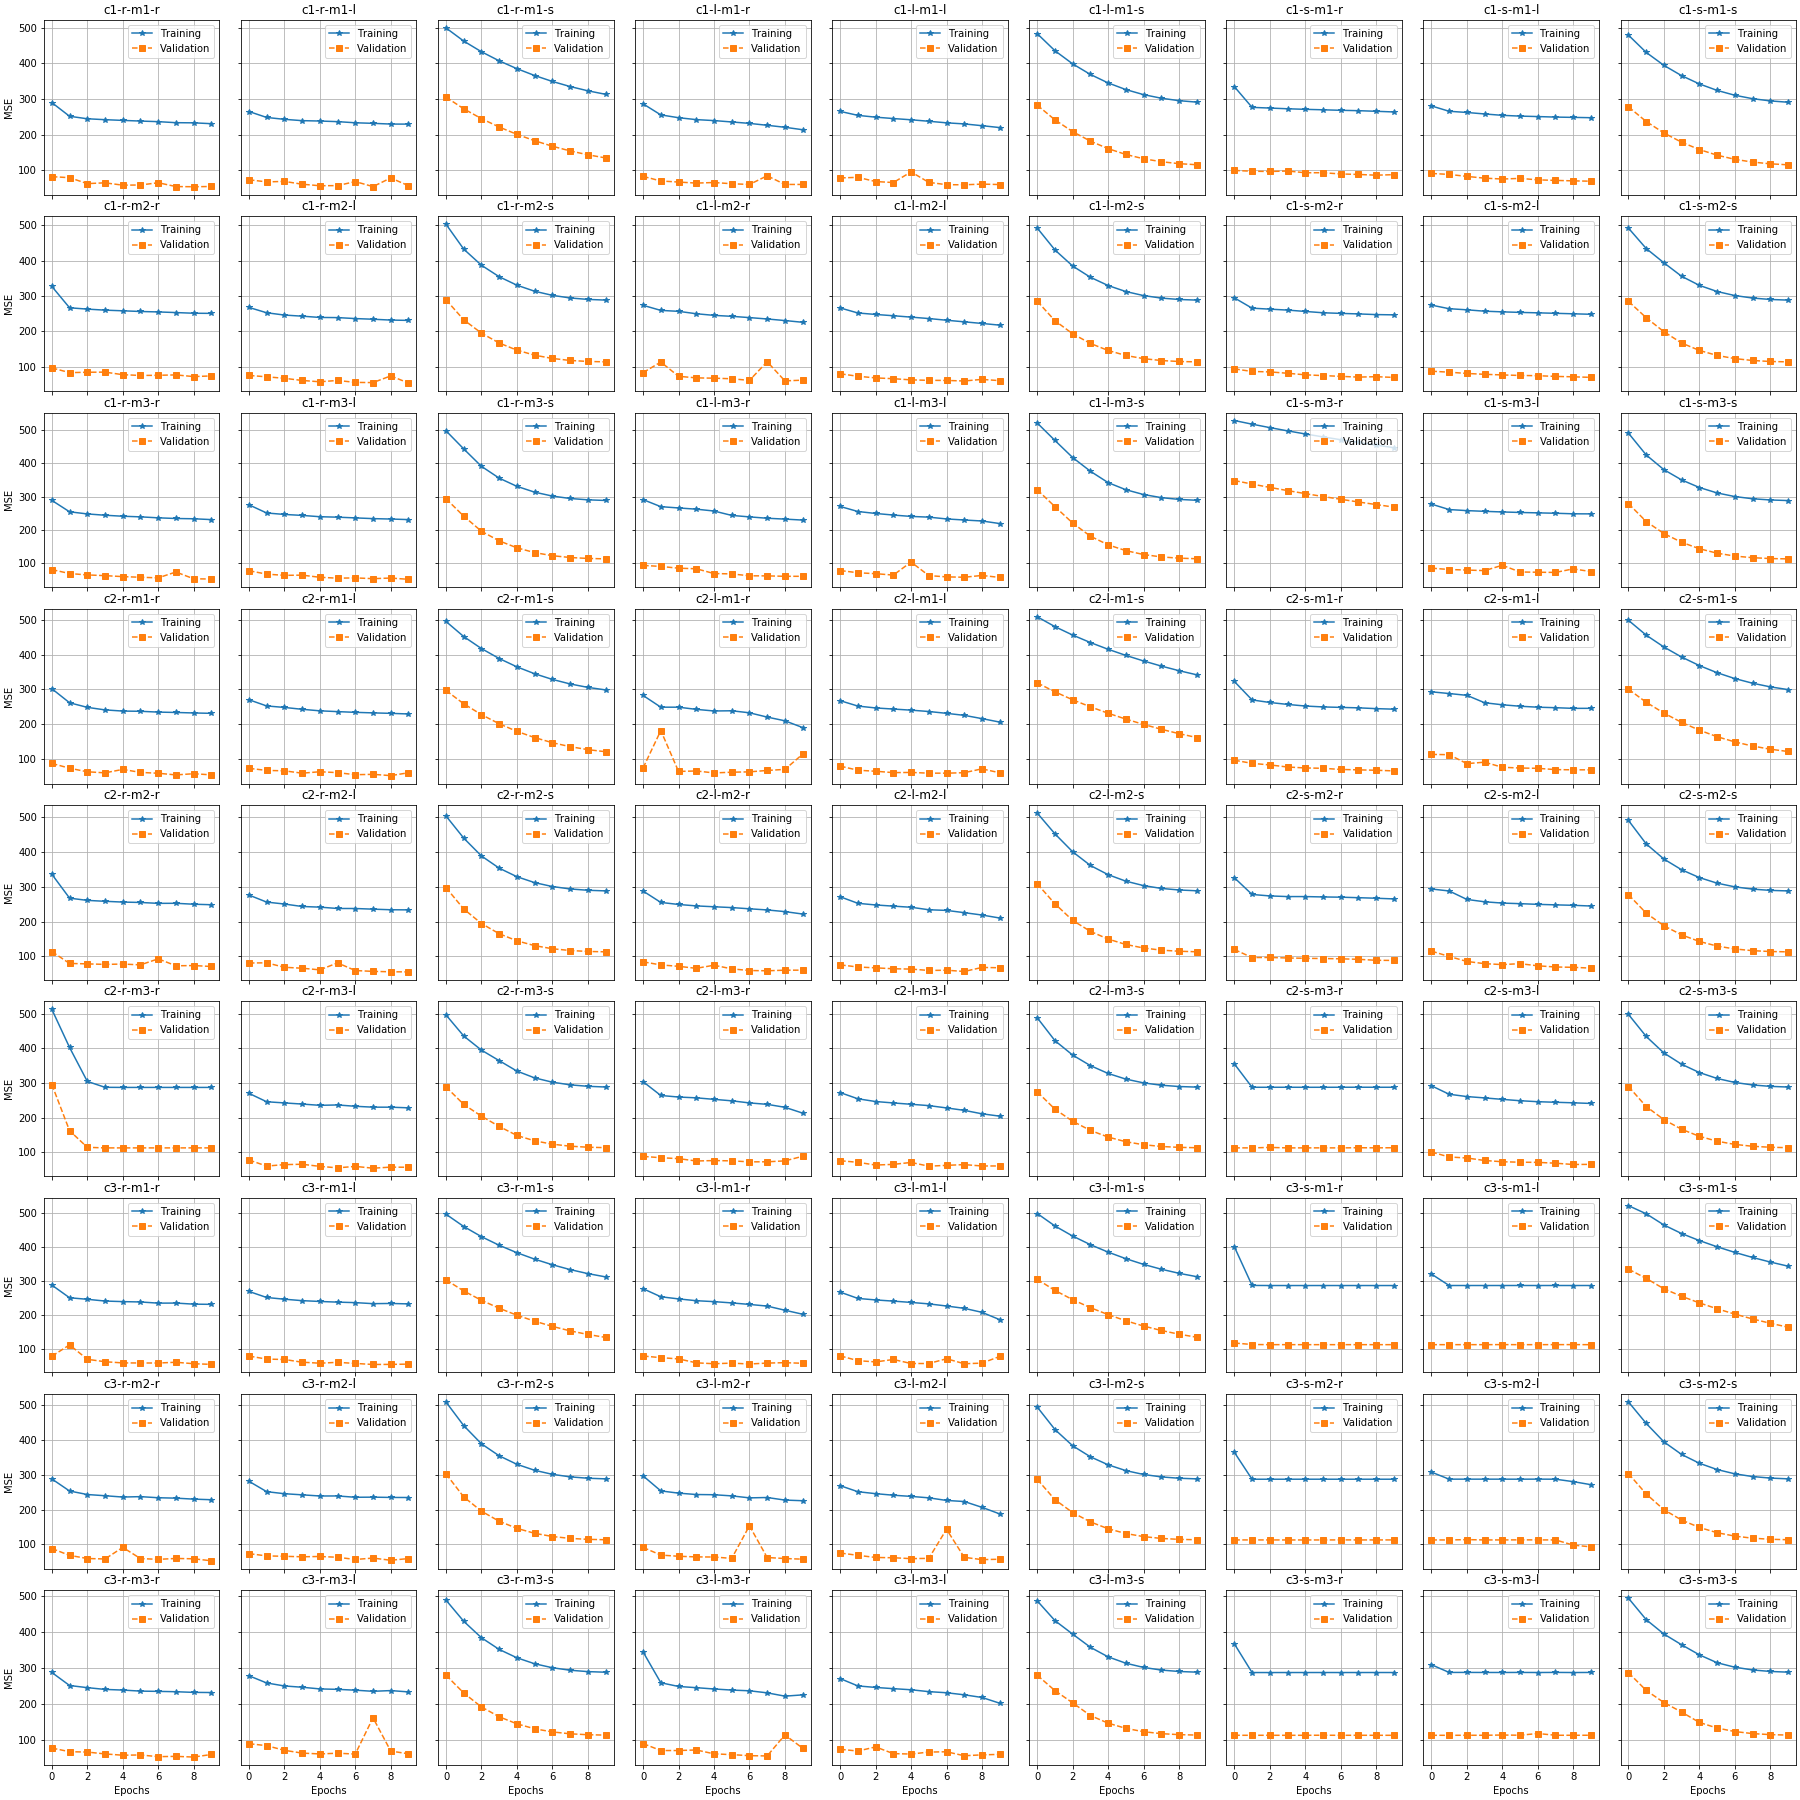
\includegraphics[width=1.0\linewidth]{images/grid-MSE-epochs-10.png}
\caption{CNN model grid search for prediction stage}
\label{fig:gridSearchCNN10epoch}
\end{figure} 


\begin{figure}
\centering
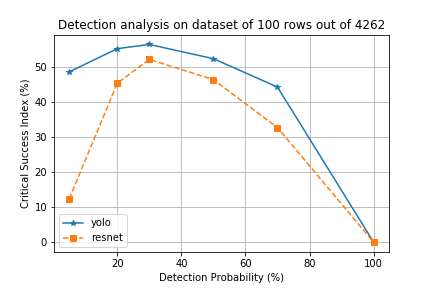
\includegraphics[width=0.8\linewidth]{images/detector_100-rows_CSI-analysis.png}
\caption{CSI analysis for both detection algorithms}
\label{fig:100rowCSI}
\end{figure} 

\begin{figure}
\centering
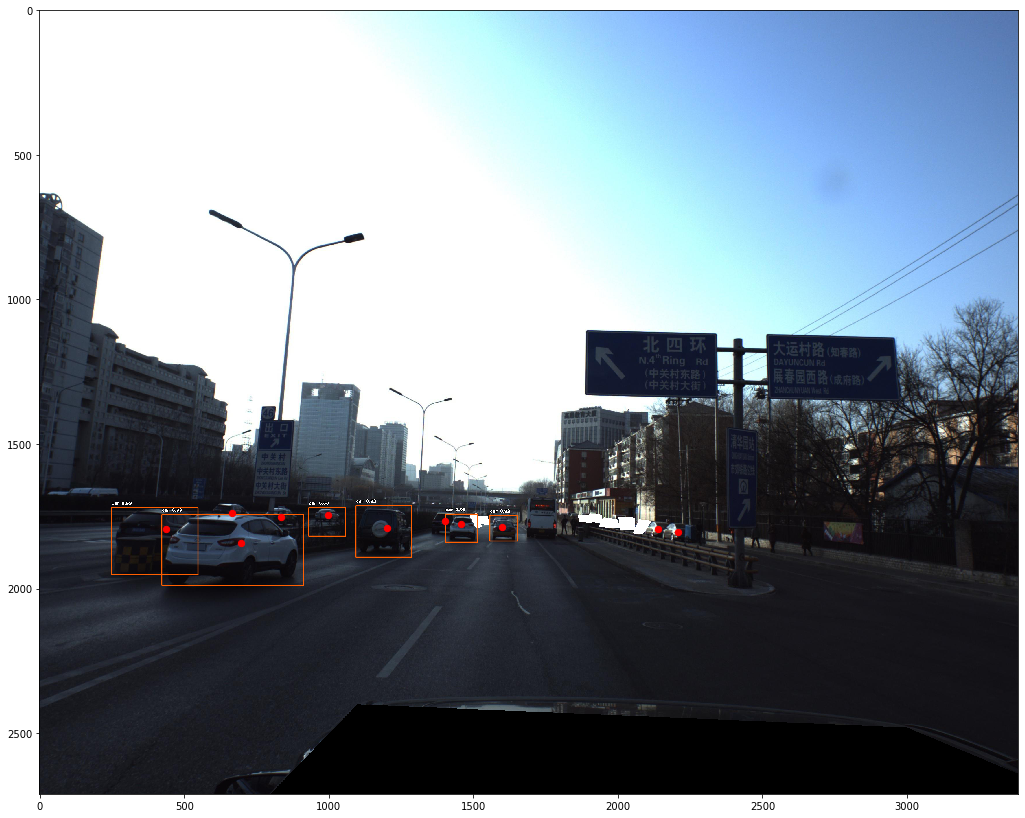
\includegraphics[width=0.8\linewidth]{images/TP-6-FP-0-FN-5.png}
\caption{Detection example 1 - image has 6 TP, 0 FP, 5 FN }
\label{fig:example6TP5FN}
\end{figure} 



\begin{figure}
\centering
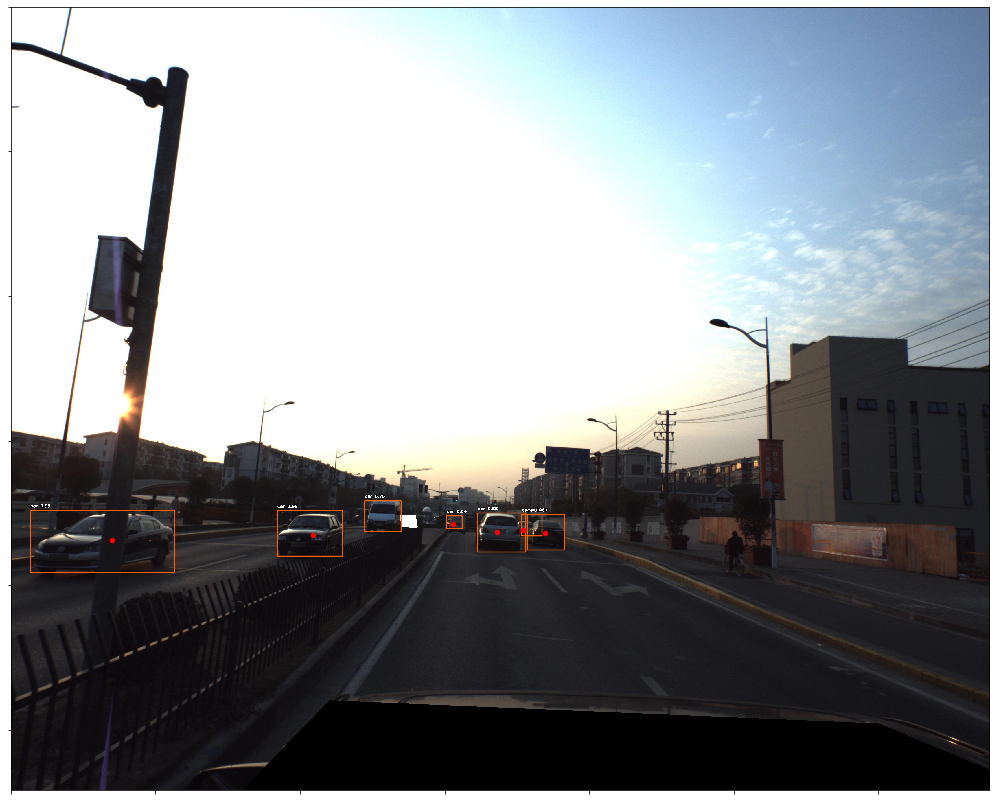
\includegraphics[width=0.8\linewidth]{images/FP-1.png}
\caption{Detection example 2 - image has 1 FP }
\label{fig:example1FP}
\end{figure} 
